% Template for Cogsci submission with R Markdown

% Stuff changed from original Markdown PLOS Template
\documentclass[10pt, letterpaper]{article}

\usepackage{cogsci}
\usepackage{pslatex}
\usepackage{float}
\usepackage{caption}

% amsmath package, useful for mathematical formulas
\usepackage{amsmath}

% amssymb package, useful for mathematical symbols
\usepackage{amssymb}

% hyperref package, useful for hyperlinks
\usepackage{hyperref}

% graphicx package, useful for including eps and pdf graphics
% include graphics with the command \includegraphics
\usepackage{graphicx}

% Sweave(-like)
\usepackage{fancyvrb}
\DefineVerbatimEnvironment{Sinput}{Verbatim}{fontshape=sl}
\DefineVerbatimEnvironment{Soutput}{Verbatim}{}
\DefineVerbatimEnvironment{Scode}{Verbatim}{fontshape=sl}
\newenvironment{Schunk}{}{}
\DefineVerbatimEnvironment{Code}{Verbatim}{}
\DefineVerbatimEnvironment{CodeInput}{Verbatim}{fontshape=sl}
\DefineVerbatimEnvironment{CodeOutput}{Verbatim}{}
\newenvironment{CodeChunk}{}{}

% cite package, to clean up citations in the main text. Do not remove.
\usepackage{apacite}

% KM added 1/4/18 to allow control of blind submission


\usepackage{color}

% Use doublespacing - comment out for single spacing
%\usepackage{setspace}
%\doublespacing


% % Text layout
% \topmargin 0.0cm
% \oddsidemargin 0.5cm
% \evensidemargin 0.5cm
% \textwidth 16cm
% \textheight 21cm

\title{How to Make a Proceedings Paper Submission}

\usepackage{float} \floatplacement{figure}{T} \usepackage{graphicx}
\usepackage{booktabs}
\usepackage{longtable}
\usepackage{array}
\usepackage{multirow}
\usepackage{wrapfig}
\usepackage{float}
\usepackage{colortbl}
\usepackage{pdflscape}
\usepackage{tabu}
\usepackage{threeparttable}
\usepackage{threeparttablex}
\usepackage[normalem]{ulem}
\usepackage{makecell}
\usepackage{xcolor}

\author{{\large \bf Morton Ann Gernsbacher (MAG@Macc.Wisc.Edu)} \\ Department of Psychology, 1202 W. Johnson Street \\ Madison, WI 53706 USA \AND {\large \bf Sharon J.~Derry (SDJ@Macc.Wisc.Edu)} \\ Department of Educational Psychology, 1025 W. Johnson Street \\ Madison, WI 53706 USA}

\newlength{\cslhangindent}
\setlength{\cslhangindent}{1.5em}
\newenvironment{CSLReferences}%
  {}%
  {\par}

\begin{document}

\maketitle

\begin{abstract}
Include no author information in the initial submission, to facilitate
blind review. The abstract should be one paragraph, indented 1/8 inch on
both sides, in 9\textasciitilde point font with single spacing. The
heading `Abstract' should be 10\textasciitilde point, bold, centered,
with one line of space below it. This one-paragraph abstract section is
required only for standard six page proceedings papers. Following the
abstract should be a blank line, followed by the header `Keywords' and a
list of descriptive keywords separated by semicolons, all in
9\textasciitilde point font, as shown below.

\textbf{Keywords:}
Add your choice of indexing terms or keywords; kindly use a semi-colon;
between each term.
\end{abstract}

\hypertarget{background}{%
\section{Background}\label{background}}

\hypertarget{basis-of-generalizations}{%
\subsection{Basis of generalizations}\label{basis-of-generalizations}}

What does ``dog'' mean to a 2-year-old? This old question reflects the
evolving nature of our understanding of early label categorization. For
young children, a dog might initially be identified by a set of
perceptual features that expands with experience (CLARK, 1973). Over
time, deeper attributes, such as its internal composition, behavior and
interaction with the world, or sound, may also become relevant (Carey,
1985). The defining features of the lexical category manifest in the way
the word is used to label other objects. Understanding how children
generalize a noun learned in the presence of a few examplars remains
critical to deciphering the underlying processes of lexical concept
formation. Overextensions are common in early word acquisition
{[}Rescorla LA. Overextension in early language development{]}, yet the
nature of the underlying representations and their developmental
trajectory remain debated. For example, The semantic features hypothesis
(CLARK, 1973) suggests that categorization begins with schemas of basic
perceptual attributes, such as {[}four legs, tail, fur{]} for dog, hence
we see overextensions of the word ``dog'' to beings that share these set
of features like cats for example. In contrast, the functional core
hypothesis (Nelson, 1974) posits that children extract probabilistic
relationships among features to identify future category members without
treating these features as defining. In this view, perceptual attributes
like {[}four legs, tail, fur{]} act as identifiers rather than
encapsulating the category's essence. Both frameworks agree, however,
that shared perceptual features facilitate identification and labeling,
forming the foundation for the well-studied shape bias Larissa K.
Samuelson \& Smith (2000).

The shape bias is a word learning constraint that is argued to
facilitate early noun acquisition, to be an important route to
vocabulary growth, and found to be weaker in children with language
delay (Jones, 2003; JONES \& SMITH, 2005; Smith, Jones, Landau,
Gershkoff-Stowe, \& Samuelson, 2002). Nevertheless, the shape bias
observed in word learning experiments is highly variable across ages,
cultures, languages, and experimental conditions, leading to conflicting
outcomes and difficulties commensurating state of evidence to form a
coherent understanding of the phenomon of label categorization. A recent
meta-analytic effect size of 0.8, derived from over 300 standardized
effects across 40 studies (Abdelrahim \& Frank, 2024), confirms the
robustness of the shape bias. However, substantial heterogeneity in the
data (with over 90\% of variance unexplained by age or language)
suggests that cross-cultural, linguistic, and developmental differences
remain masked.

\hypertarget{sources-of-heterogeneity}{%
\subsection{Sources of Heterogeneity}\label{sources-of-heterogeneity}}

\hypertarget{task-format}{%
\subsubsection{Task format}\label{task-format}}

Generalization in word learning is often assessed using the word
extension task. Here, children are taught a novel label for a novel
object and tested on their ability to extend it to other objects that
share features like shape, or material, etc, with the exemplar object.
Word extensions are often measured via Forced-choice tasks, which
require restrictive generalizations, yes/no endorsement tasks, allowing
broader acceptance of category membership which allows for different
levels of similarity and difference (cite), or Open-choice tasks,
enabling children to reject all options, assumed to indicate an
understanding of category membership that goes beyond shared perceptual
features (Cimpian et al 2005). Forced-choice tasks may yield different
results compared to yes/no endorsement tasks, and allowing children to
select ``none of those'' reduces shape bias, especially with complex
objects (Cimpian, 2005). The choice of the task format is often guided
by the theoretical framework of the researchers, leading to what seems
like a circular stream of events in which theory informs task selection,
and task selection confirms theory.

\hypertarget{stimuli}{%
\subsubsection{Stimuli}\label{stimuli}}

A significant sources of variation in the word extension findings comes
from differences in stimuli. Just like task format, these methodological
decisions are often driven by theoretical frameworks as well. For
instance, studies focusing on low-level attentional biases typically
emphasize contrasts between shape and other perceptual features, such as
color or material, using stimuli designed to highlight these attributes.
On the other hand, studies investigating conceptual understanding often
include cues related to animacy, such as eyes, shoes, or other salient
features, and use test objects that share multiple dimensions with the
exemplar instead of only one to explore broader conceptual frameworks
(cite). When functionality is emphasized, stimuli are often paired with
demonstrations of an affordance, stories, or narratives to contrast
shape with function. Children aged {[}X--Y{]} are frequently found to
prioritize shape, even when provided with functional information
(Gentner \& Rattermann, 1991; Woodward \& Markman, 1998; etc.). However,
conflicting evidence shows children sometimes prioritize function or
other cues (Kemler Nelson, 1995; Gelman \& Medin, 1993; etc.), with
variation linked to factors like whether test objects were handled or
how stimuli were designed (e.g., functional bases vs.~appended parts).
In addition, some studies use pictures or drawings, while others use
physical objects (cite).

Lastly, most studies employ between-subjects designs, which do not
control for individual differences, further amplifying heterogeneity.
These procedural and stimuli variations reflect broader theoretical
questions about the origins of the shape bias (Smith \& Medin, 1981). Is
it a Low-level attentional mechanisms driven by attentional processes
that guide children to perceptual features associated with category
labels? Or a Top-down conceptual processes in which the perceptual
features act as identifiers rather than defining properties? Where
should the line be drawn between perceptual feature identification and
the core representation of conceptual labels? Are these separate
processes, or do they exist on a continuum that develops as children
acquire more information? How do attention to perceptual attributes and
conceptual understanding interact during development (Madole \& Oakes,
1999)? These foundational questions influence procedural decisions and
should be kept in mind when investigating label categorization and
concept formation.

\hypertarget{theorectical-implications}{%
\section{Theorectical implications}\label{theorectical-implications}}

The investigation of the shape bias, and label categorization more
broadly, has unfolded around two major debates: a cross-cultural debate
and a representational debate.

\hypertarget{cross-linguistic-debate}{%
\subsection{Cross-linguistic debate}\label{cross-linguistic-debate}}

The word extension task literature highlights significant
cross-linguistic differences in the prevalence of the shape bias, which
are considered theoretically important. For example, speakers of East
Asian languages like Mandarin and Japanese demonstrate less reliance on
shape when extending nouns compared to English speakers in the United
States (Gathercole, 1997; Imai \& Gentner, 1997; Samuelson \& Smith,
1999; Soja et al., 1991; Subrahmanyam \& Chen, 2006; Yoshida \& Smith,
2003). (Gathercole \& Min (1997); Imai \& Gentner (1997); Larissa K.
Samuelson \& Smith (1999); Nancy N. Soja, Carey, \& Spelke (1991);
Subrahmanyam \& Chen (2006); Yoshida \& Smith (2003b)).

Two key hypotheses attempt to explain these differences: 1- Syntactic
Structure Hypothesis: Differences in linguistic structure, such as
count-mass syntax in English versus classifier systems in East Asian
languages, influence the prevalence of the shape bias (Larissa K.
Samuelson, Horst, Schutte, \& Dobbertin (2008); Nancy N. Soja et al.
(1991); Nancy N. Soja, Carey, \& Spelke (1992))

2- Statistical Regularities Hypothesis: Variations in lexical and
environmental statistical regularities tunes attention toward features
like shape. This hypothesis emphasizes the role of existing vocabulary
and environmental exposure in guiding category organization
(Gershkoff-Stowe \& Smith (2004); Larissa K. Samuelson (2002); Larissa
K. Samuelson \& Smith (1999); Perry, Samuelson, Malloy, \& Schiffer
(2010); Colunga \& Smith (2000); Yoshida \& Smith (2003a),
Jara-Ettinger, Levy, Sakel, Huanca, \& Gibson (2022); Abdelrahim \&
Frank (2024))

\hypertarget{the-perception-or-conception-debate}{%
\subsection{The Perception or conception
debate}\label{the-perception-or-conception-debate}}

A second key debate focuses on the mechanism or representation
underlying the shape bias. While the tendency to extend nouns based on
shape may be influenced by syntax or statistical regularities, its
precise cognitive basis has been controversial (Smith et al. (2002);
Smith, Colunga, \& Yoshida (2010); Brady \& Chun, 2007; Chun \& Jiang,
1998).

Two competing perspectives attempt to explain this mechanism:

1- Associative and Non-Strategic Mechanism: The shape bias is viewed as
an early cognitive tool, helping children ``break into'' language by
rapidly mapping nouns to referents through associative processes. This
bias operates on a perceptual level, organizing categories around
salient features like shape. For instance, the shape of a dog becomes
synonymous with the category ``dog.'' This view posits that the bias is
non-strategic, independent of conceptual understanding or general world
knowledge (Smith et al., 2002; Smith \& Colunga, 2010; Brady \& Chun,
2007; Chun \& Jiang, 1998).

2- Strategic and Conceptually Controlled Mechanism: The shape bias is
seen as a flexible and controlled process, governed by general world
knowledge and conceptual understanding. In this framework, the bias is a
heuristic that can be overridden when context or conceptual goals
require attention to other features, such as function.

\hypertarget{the-nature-of-knowledge}{%
\subsection{The nature of Knowledge}\label{the-nature-of-knowledge}}

Given that task design is influenced by theoretical assumptions, this
raises another important question: What type of knowledge do these tasks
measure? Two key assumptions can stem out of this: Knowledge as Stable
and Fixed: If knowledge is stable, tasks merely elicit pre-existing
constructs. Investigating heterogeneity would then focus on ensuring
task validity and reliability in capturing the theoretical construct.
Knowledge as Dynamic and Task-Dependent: If knowledge is dynamic,
categorization depends on the interaction between task specifics and
children's behavior. This view suggests that children dynamically select
information sources to organize categories, influenced by the context of
the task and the nature of the stimuli (Smith et al., 2010). If the
second assumption holds, achieving consistency in measures across
studies is crucial to isolating the relevant contextual cues that tasks
provide specially for cross-cultural studies that aim to adjudicate
theoretical debates.

Regardless of which assumption holds, it is necessary to evaluate the
heterogeneity in the word categorization studies which highlights the
importance of methodological consistency and the need to consider the
theoretical premises underlying procedural decisions. Understanding how
these premises shape task designs and influence results is key to
advancing our knowledge of label categorization and concept formation.

\hypertarget{current-study}{%
\section{Current Study}\label{current-study}}

This project attempts to provide a first step into a larger scale
assessment of word generalization across age groups and languages. The
main goal of this study is to evaluate the effect of procedural design
and stimuli design on the heterogeneity seen in word generalization
tasks. We utilize a within-subject design, controlling for individual
differences which we believe is important for a proper comparison
between conditions that require giving different instructions and cues
to the participants. We aim to recruit a larger sample size of a wider
age group, with a variety of items and test trials. Given our focus on
early language acquisition and the noun bias dominating early vocabulary
(cite), we prioritize studies examining functional information over
other types of conceptual knowledge.

\hypertarget{stimuli-design}{%
\subsection{Stimuli design}\label{stimuli-design}}

Seven stimuli sets were hand crafted such that each set contains one
exemplar, a material match, a shape match, a function match, and a
distractor. In experiment 1, the shape match is contrasted with a
material match, it served as a basic check and a replication of previous
findings, while in experiment 2, the shape match is contrasted with a
function match. The same exemplar is used in both experiments, and color
is not shared across any of the objects. For the function test object,
it is modified in a way that doesn't change the shape at all, but allows
for the function (i.e.~an object that is wrapped all over and a similar
one that can clearly open). Objects are designed in a way that can
answer to questions of how much children reason about the whole vs parts
similarity, how they reason about material, and the influence of
previous experiences with objects (see suplementary) ( cite Neslon and
graham and ).

\hypertarget{adults-ratings}{%
\subsection{Adults ratings}\label{adults-ratings}}

\hypertarget{experiment-1-a-preliminary}{%
\subsection{Experiment 1: a
preliminary}\label{experiment-1-a-preliminary}}

\hypertarget{participants}{%
\subsubsection{Participants}\label{participants}}

Twenty four typically developing English speaking participants (2-5
years old, mean=44.05, SD=15.29) were recruited from a local nursery
school and children's museum in the US.

\hypertarget{procedure}{%
\subsubsection{Procedure}\label{procedure}}

Seven trials were conducted in which each participant sees an object
being labeled ``this is a dax'', the object is taken away but still in
view, both test objects and the distractor are displayed simultaneously
while asking the child ``can you find another dax by pointing to it?''.
The child gets to hear the label 3 times while viewing it without
touching it.

\hypertarget{results}{%
\subsubsection{Results}\label{results}}

\begin{CodeChunk}
\begin{figure}[tb]
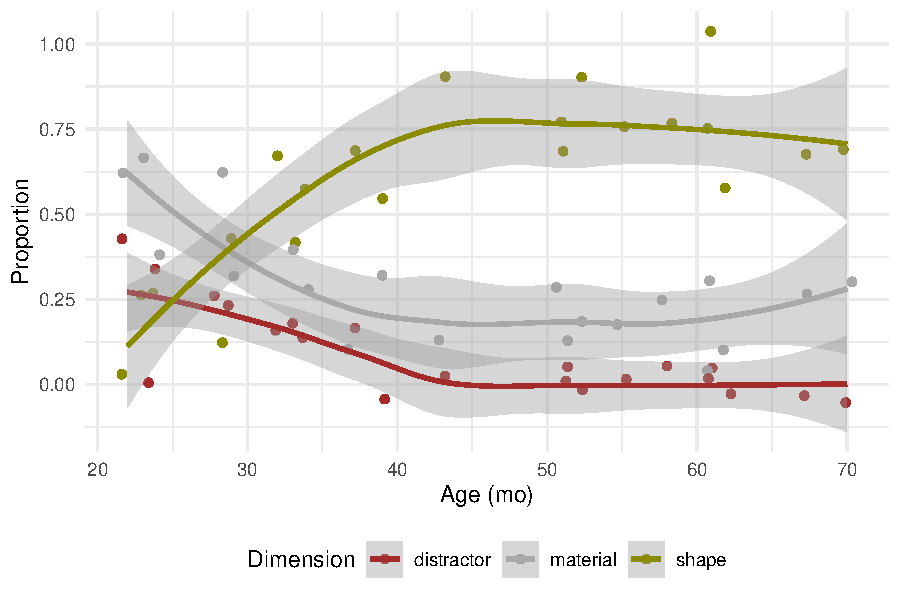
\includegraphics[width=1\linewidth]{figs/first_exp-1} \caption[some caption here]{some caption here}\label{fig:first_exp}
\end{figure}
\end{CodeChunk}

Participants showed an overall shape bias across all trials (shape:61\%,
material:30\%, distractor: 9\%). Figure \ref{fig:first_exp} shows a
developmental shift to choose by shape by age 3, replicating what is
seen previously in the literature.\\
A generalized logistic mixed-effects model (GLMM) reveals an average
intercept odds of 0.11 (odds of 0.11:1 at the mean age, \(p=\)
\textless{} .001), with a significant increase in odds of 1.06 per unit
increase in age (\(p=\) \textless{} .001). The model also shows
variability at the item-level intercept (variance = 0.11, SD = 0.32)
across 7 unique items (standardlabel groups). After replicating the
shape bias effect using the set of stimuli we created in a simple set
up, our next experiment explores an design that tests for both
conditions when shape is only contrasted with material without any
additional information, and a condition in which shape is contrasted
with function after demonstrating the function for the exemplar, while
controlling for individual differences with a bigger sample size to
capture variability at the item level.

\hypertarget{experiment-2}{%
\subsection{Experiment 2}\label{experiment-2}}

\hypertarget{participants-1}{%
\subsubsection{Participants}\label{participants-1}}

31 (target n=96, 24 per each age group) participants between 2-5 years
old (mean=48.22, SD=5.54, n per age group) were recruited from a local
nursery school in the US.

\hypertarget{procedure-1}{%
\subsubsection{Procedure}\label{procedure-1}}

A within subject manipulation with two conditions: material or function.
The material condition is identical to the first experiment. In the
function condition, the experimenter introduce the exemplar object
``this is a dax'', gives the child 15 seconds seconds to play with it,
provides functional information `` the dax grapes toys'', gives another
15 seconds to play with it, and puts the toy away but within view,
before introducing the test objects and asks for a response.

\begin{CodeChunk}
\begin{figure*}[tb]
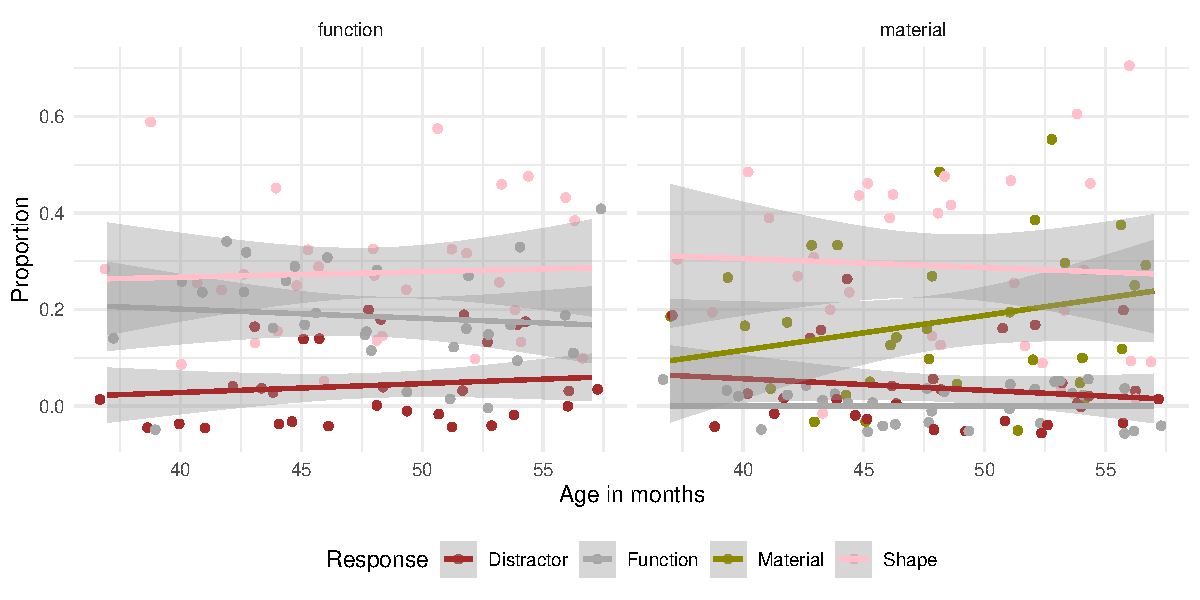
\includegraphics[width=1\linewidth]{figs/jitter_function-1} \caption[some caption here]{some caption here}\label{fig:jitter_function}
\end{figure*}
\end{CodeChunk}

\hypertarget{preliminary-results}{%
\subsubsection{Preliminary results}\label{preliminary-results}}

Similar to what is conveyed in Figure \ref{fig:jitter_function}, A
generalized logistic mixed-effects model (GLMM) showed baseline odds of
2.25 (odds of 2.25:1 for the function condition \(p=\) .693). The odds
increase with age by a factor of 1.01 (\(p=\) .742). While The odds for
the ``material'' condition are 0.07 times lower than for the
``function'' condition (\(p=\) .338). Additionally, the interaction
between age and condition shows that for the ``material'' condition, the
odds decrease by a factor of 0.94 per unit increase in age (\(p=\)
.294). Random effects indicate variability in intercepts across
participants (SD = 0.22) and across items (SD = 1.38) for 31
participants and 7 items. Notably, the confidence intervals show
uncertainty however data collection is still ongoing.

\hypertarget{discussion}{%
\section{Discussion}\label{discussion}}

The word extension and category organization literature is highly
heterogeneous. Studies in this domain lack an integrative and
commensurable design, which hinders our ability to draw consistent
conclusions. To achieve a more accurate measurement of category
organization and concept learning, we need a reliable and valid wide
range set of stimuli objects, consistent task formats and test designs,
as well as multi-site cross-cultural experiments unified across
laboratories to maximally account for the variability. Our evaluation of
the word extension literature reveals that making procedural decisions,
which we think are likely a primary source of unexplained variability,
is unattianable without running a series of controlled experiments that
would allow us to systematically assess how different designs and
stimuli covary with response patterns. In our initial results, we see a
strong tendency to generalize by shape, even in conditions designed to
make function salient. This suggests that, even with a potential
saliency effect, where the trials highlighted functional information, it
failed to override the preference for shape-based choices. In additon,
many children explored whether their chosen test object could perform
the intended function after selecting it based on shape. This behavior
implies that the shape-based selection might not reflect a disregard for
functional information but rather a hypothesis that objects sharing
shape might also share functionality.

EDIT: What does it mean to talk about validity and reliability in a task
like the word extension one? What is the construct we are talking about
here. It is a measure at the group level rather than at the individual
level \textgreater\textgreater{} this kid had this level of shape bias.
\textgreater\textgreater{} is it an issue of the signal is not even
there, or is it a matter of the level/degree of the signal when it comes
to cross-cultural work. (Madole, K. L., \& Oakes, L. M. (1999)):
Although the distinction between perceptual and conceptual categories
makes a certain intuitive sense, it may only confuse our attempts to
understand psychological reality. Establishing a reliable metric for
this distinction is extremely difficult and attempts to operationalize
the terms perceptual and conceptual are invariably highly ambiguous and
task-specific. How the perceptual vs conceptual debate maps into the
cross cultural differences debate ? As we mentioned in the introduction,
procedural variation observed in the literature have followed
theoretical debates and in fact reinforced by them. Thus, evaluating the
theories given the state of evidence is not feasbile and it will endup
crashing with this heterogeneity and with the broader question on the
type of knowledge being highlighted by each one of the evidence.

\hypertarget{references}{%
\section{References}\label{references}}

\setlength{\parindent}{-0.1in} 
\setlength{\leftskip}{0.125in}

\noindent

\hypertarget{refs}{}
\begin{CSLReferences}{1}{0}
\leavevmode\vadjust pre{\hypertarget{ref-abdelrahim_frank_2024}{}}%
Abdelrahim, S., \& Frank, M. C. (2024, September). Examining the
robustness and generalizability of the shape bias: A meta-analysis.
PsyArXiv.
http://doi.org/\href{https://doi.org/10.31234/osf.io/3by54}{10.31234/osf.io/3by54}

\leavevmode\vadjust pre{\hypertarget{ref-Baldwin1992ClarifyingTR}{}}%
Baldwin, D. A. (1992). Clarifying the role of shape in children's
taxonomic assumption. \emph{Journal of Experimental Child Psychology},
\emph{54 3}, 392--416. Retrieved from
\url{https://api.semanticscholar.org/CorpusID:29725812}

\leavevmode\vadjust pre{\hypertarget{ref-CLARK197365}{}}%
CLARK, E. V. (1973). WHAT's IN a WORD? ON THE CHILD's ACQUISITION OF
SEMANTICS IN HIS FIRST LANGUAGE11This research was supported in part by
NSF grant GS-1880 to the language universals project, stanford
university, and in part by NSF grant GS-30040 to the author. In T. E.
Moore (Ed.), \emph{Cognitive development and acquisition of language}
(pp. 65--110). San Diego: Academic Press.
http://doi.org/\url{https://doi.org/10.1016/B978-0-12-505850-6.50009-8}

\leavevmode\vadjust pre{\hypertarget{ref-colunga2000learning}{}}%
Colunga, E., \& Smith, L. B. (2000). Learning to learn words: A
cross-linguistic study of the shape and material biases. In
\emph{Proceedings of the 24th annual boston university conference on
language development} (Vol. 1, pp. 197--207).

\leavevmode\vadjust pre{\hypertarget{ref-gathercole_1997}{}}%
Gathercole, V. C. M., \& Min, H. (1997). Word meaning biases or
language-specific effects? {Evidence} from {English}, {Spanish} and
{Korean}. \emph{First Language}, \emph{17}(51), 031--56.
http://doi.org/\href{https://doi.org/10.1177/014272379701705102}{10.1177/014272379701705102}

\leavevmode\vadjust pre{\hypertarget{ref-gershkoff2004shape}{}}%
Gershkoff-Stowe, L., \& Smith, L. B. (2004). Shape and the first hundred
nouns. \emph{Child Development}, \emph{75}(4), 1098--1114.

\leavevmode\vadjust pre{\hypertarget{ref-graham_2010}{}}%
Graham, S. A., \& Diesendruck, G. (2010). Fifteen-month-old infants
attend to shape over other perceptual properties in an induction task.
\emph{Cognitive Development}, \emph{25}(2), 111--123.
http://doi.org/\href{https://doi.org/10.1016/j.cogdev.2009.06.002}{10.1016/j.cogdev.2009.06.002}

\leavevmode\vadjust pre{\hypertarget{ref-Graham1999InfantsRO}{}}%
Graham, S. A., \& Poulin-Dubois, D. (1999). Infants' reliance on shape
to generalize novel labels to animate and inanimate objects.
\emph{Journal of Child Language}, \emph{26}, 295--320. Retrieved from
\url{https://api.semanticscholar.org/CorpusID:43424185}

\leavevmode\vadjust pre{\hypertarget{ref-imai1997}{}}%
Imai, M., \& Gentner, D. (1997). A cross-linguistic study of early word
meaning: Universal ontology and linguistic influence. \emph{Cognition},
\emph{62}(2), 169--200.

\leavevmode\vadjust pre{\hypertarget{ref-imai_childrens_1994}{}}%
Imai, M., Gentner, D., \& Uchida, N. (1994). Children's theories of word
meaning: {The} role of shape similarity in early acquisition.
\emph{Cognitive Development}, \emph{9}(1), 45--75.
http://doi.org/\href{https://doi.org/10.1016/0885-2014(94)90019-1}{10.1016/0885-2014(94)90019-1}

\leavevmode\vadjust pre{\hypertarget{ref-jara2022}{}}%
Jara-Ettinger, J., Levy, R., Sakel, J., Huanca, T., \& Gibson, E.
(2022). The origins of the shape bias: Evidence from the tsimane'.
\emph{Journal of Experimental Psychology: General}.

\leavevmode\vadjust pre{\hypertarget{ref-Jones2003}{}}%
Jones, S. S. (2003). Late talkers show no shape bias in a novel name
extension task. \emph{Developmental Science}, \emph{6}(5), 477--483.
http://doi.org/\url{https://doi.org/10.1111/1467-7687.00304}

\leavevmode\vadjust pre{\hypertarget{ref-JONES_SMITH_2005}{}}%
JONES, S. S., \& SMITH, L. B. (2005). Object name learning and object
perception: A deficit in late talkers. \emph{Journal of Child Language},
\emph{32}(1), 223--240.
http://doi.org/\href{https://doi.org/10.1017/S0305000904006646}{10.1017/S0305000904006646}

\leavevmode\vadjust pre{\hypertarget{ref-LANDAU1988299}{}}%
Landau, B., Smith, L. B., \& Jones, S. S. (1988). The importance of
shape in early lexical learning. \emph{Cognitive Development},
\emph{3}(3), 299--321.
http://doi.org/\url{https://doi.org/10.1016/0885-2014(88)90014-7}

\leavevmode\vadjust pre{\hypertarget{ref-Nelson1974ConceptWA}{}}%
Nelson, K. (1974). Concept, word, and sentence: Interrelations in
acquisition and development. \emph{Psychological Review}, \emph{81},
267--285. Retrieved from
\url{https://api.semanticscholar.org/CorpusID:143965074}

\leavevmode\vadjust pre{\hypertarget{ref-perry2010learn}{}}%
Perry, L. K., Samuelson, L. K., Malloy, L. M., \& Schiffer, R. N.
(2010). Learn locally, think globally: Exemplar variability supports
higher-order generalization and word learning. \emph{Psychological
Science}, \emph{21}(12), 1894--1902.

\leavevmode\vadjust pre{\hypertarget{ref-samuelson_statistical_2002}{}}%
Samuelson, Larissa K. (2002). Statistical regularities in vocabulary
guide language acquisition in connectionist models and 15-20-month-olds.
\emph{Developmental Psychology}, \emph{38}(6), 1016--1037.
http://doi.org/\href{https://doi.org/10.1037/0012-1649.38.6.1016}{10.1037/0012-1649.38.6.1016}

\leavevmode\vadjust pre{\hypertarget{ref-samuelson2008rigid}{}}%
Samuelson, Larissa K., Horst, J. S., Schutte, A. R., \& Dobbertin, B. N.
(2008). Rigid thinking about deformables: Do children sometimes
overgeneralize the shape bias? \emph{Journal of Child Language},
\emph{35}(3), 559--589.

\leavevmode\vadjust pre{\hypertarget{ref-samuelson1999}{}}%
Samuelson, Larissa K., \& Smith, L. B. (1999). Early noun vocabularies:
Do ontology, category structure and syntax correspond? \emph{Cognition},
\emph{73}(1), 1--33.

\leavevmode\vadjust pre{\hypertarget{ref-samuelson2000children}{}}%
Samuelson, Larissa K., \& Smith, L. B. (2000). Children's attention to
rigid and deformable shape in naming and non-naming tasks. \emph{Child
Development}, \emph{71}(6), 1555--1570.

\leavevmode\vadjust pre{\hypertarget{ref-smithcolunga2010}{}}%
Smith, L. B., Colunga, E., \& Yoshida, H. (2010). Knowledge as process:
Contextually cued attention and early word learning. \emph{Cognitive
Science}, \emph{34}(7), 1287--1314.
http://doi.org/\url{https://doi.org/10.1111/j.1551-6709.2010.01130.x}

\leavevmode\vadjust pre{\hypertarget{ref-smith_object_2002}{}}%
Smith, L. B., Jones, S. S., Landau, B., Gershkoff-Stowe, L., \&
Samuelson, L. (2002). Object name learning provides on-the-job training
for attention. \emph{Psychological Science}, \emph{13}(1), 13--19.
http://doi.org/\href{https://doi.org/10.1111/1467-9280.00403}{10.1111/1467-9280.00403}

\leavevmode\vadjust pre{\hypertarget{ref-soja1991ontological}{}}%
Soja, Nancy N., Carey, S., \& Spelke, E. S. (1991). Ontological
categories guide young children's inductions of word meaning: Object
terms and substance terms. \emph{Cognition}, \emph{38}(2), 179--211.

\leavevmode\vadjust pre{\hypertarget{ref-soja_perception_1992}{}}%
Soja, Nancy N., Carey, S., \& Spelke, E. S. (1992). Perception,
ontology, and word meaning. \emph{Cognition}, \emph{45}(1), 101--107.
http://doi.org/\href{https://doi.org/10.1016/0010-0277(92)90025-D}{10.1016/0010-0277(92)90025-D}

\leavevmode\vadjust pre{\hypertarget{ref-subrahmanyam_2006}{}}%
Subrahmanyam, K., \& Chen, H.-H. N. (2006). A crosslinguistic study of
children's noun learning: {The} case of object and substance words.
\emph{First Language}, \emph{26}(2), 141--160.
http://doi.org/\href{https://doi.org/10.1177/0142723706060744}{10.1177/0142723706060744}

\leavevmode\vadjust pre{\hypertarget{ref-yoshida2003known}{}}%
Yoshida, H., \& Smith, L. B. (2003a). Known and novel noun extensions:
Attention at two levels of abstraction. \emph{Child Development},
\emph{74}(2), 564--577.

\leavevmode\vadjust pre{\hypertarget{ref-yoshida2003}{}}%
Yoshida, H., \& Smith, L. B. (2003b). Shifting ontological boundaries:
How japanese-and english-speaking children generalize names for animals
and artifacts. \emph{Developmental Science}, \emph{6}(1), 1--17.

\end{CSLReferences}

\bibliographystyle{apacite}


\end{document}
